%%% Econ717: Applied Econometrics
%%% Spring 2022
%%% Danny Edgel
%%%
% Due on Canvas Monday, March 28th, 11:00 AM
%%%

%%%
%							PREAMBLE
%%%

\documentclass{article}

%%% declare packages
\usepackage{amsmath}
\usepackage{amssymb}
\usepackage{array}
\usepackage{bm}
\usepackage{bbm}
\usepackage{changepage}
\usepackage{centernot}
\usepackage{color}
\usepackage{courier}
\usepackage{graphicx}
\usepackage{listings}
\usepackage[shortlabels]{enumitem}
\usepackage{boondox-cal}
\usepackage{fancyhdr}
	\fancyhf{} % sets both header and footer to nothing
	\renewcommand{\headrulewidth}{0pt}
    \rfoot{Edgel, \thepage}
    \pagestyle{fancy}
	
%%% define shortcuts for set notation
\newcommand{\N}{\mathcal{N}}
\newcommand{\Z}{\mathbb{Z}}
\newcommand{\R}{\mathbb{R}}
\newcommand{\Q}{\mathbb{Q}}
\newcommand{\union}{\bigcup}
\newcommand{\intersect}{\bigcap}
\newcommand{\lmt}{\underset{x\rightarrow\infty}{\text{lim }}}
\newcommand{\neglmt}{\underset{n\rightarrow-\infty}{\text{lim }}}
\newcommand{\zerolmt}{\underset{x\rightarrow 0}{\text{lim }}}
\newcommand{\usmax}{\underset{1\leq k \leq n}{\text{max }}}
\newcommand{\usmin}[1]{\underset{#1}{\text{min }}}
\newcommand{\intinf}{\int_{-\infty}^{\infty}}
\newcommand{\olx}[1]{\overline{X}_{#1}}
\newcommand{\oly}[1]{\overline{Y}_{#1}}
\newcommand{\olz}[1]{\overline{Z}_{#1}}
%\newcommand{\est}[1]{\frac{1}{#1}\sum_{i=1}^{#1}}
\newcommand{\est}[1]{\frac{1}{\lowercase{#1}}\sum_{i=1}^{\lowercase{#1}}}
\newcommand{\sumn}{\sum_{i=1}^{n}}
\newcommand{\loge}[1]{\text{log}\left(#1\right)}
\renewcommand{\tilde}[1]{\widetilde{#1}}
\newcommand{\tb}{\tilde{\beta}}
\renewcommand{\Pr}[1]{\text{Pr}\left(#1\right)}
\newcommand{\bols}{\hat{\beta}^{OLS}}
\newcommand{\bhat}{\hat{\beta}}
\newcommand{\ahat}{\hat{\alpha}}
\newcommand{\ehat}{\hat{\varepsilon}}
\newcommand{\vols}{\hat{\varepsilon}_{OLS}}
\newcommand{\one}[1]{\mathbbm{1}\left\{#1\right\}}
\newcommand{\tr}[1]{\text{tr}\left(#1\right)}
\newcommand{\pfrac}[2]{\left(\frac{#1}{#2}\right)}
\newcommand{\bcls}{\tilde{\beta}_{CLS}}
\renewcommand{\L}{\mathcal{L}}
\newcommand{\vt}{\tilde{\varepsilon}}
\renewcommand{\Pr}[1]{Pr\left(#1\right)}
\newcommand{\biv}{\bhat^{IV}}
\newcommand{\xbar}{\overline{X}}
\newcommand{\ybar}{\overline{Y}}
\newcommand{\zbar}{\overline{Z}}
\newcommand{\eps}{\varepsilon}
\newcommand{\esti}{\frac{1}{T_i-1}\sum_{t=1}^{T_i}}
\newcommand{\oinv}{\Omega^{-1}}
\newcommand{\olg}{\overline{g}_n}
\newcommand{\e}[1]{\text{exp}\left(#1\right)}
\DeclareRobustCommand{\bbone}{\text{\usefont{U}{bbold}{m}{n}1}}
\newcommand{\that}{\hat{\theta}_n}
\newcommand{\tshat}{\hat{\theta}^*_n}
\newcommand{\ttilde}{\tilde{\theta}_n}
\newcommand{\ghat}{\hat{\gamma}_n}
\newcommand{\gtilde}{\tilde{\gamma}_n}
\newcommand{\chat}{\hat{c}}
\newcommand{\Qhat}{\hat{Q}_n(\beta)}
\renewcommand{\lim}[1]{\underset{#1}{\text{lim }}}
\newcommand{\xs}{X^*}
\newcommand{\olxs}{\overline{X}^*}
\newcommand{\pinv}{\Phi^{-1}}
\newcommand{\tchat}{\that^\dagger}

\newcommand{\E}[1]{\mathbb{E}\left[#1\right]}% expected value
\newcommand{\Es}[1]{\mathbb{E}^*\left[#1\right]}% expected value
\renewcommand{\exp}[1]{\E\left[#1\right]}

\definecolor{mygreen}{RGB}{28,172,0} % color values Red, Green, Blue
\definecolor{mylilas}{RGB}{170,55,241}


%%% define column vector command (from Michael Nattinger)
\newcount\colveccount
\newcommand*\colvec[1]{
        \global\colveccount#1
        \begin{pmatrix}
        \colvecnext
}
\def\colvecnext#1{
        #1
        \global\advance\colveccount-1
        \ifnum\colveccount>0
                \\
                \expandafter\colvecnext
        \else
                \end{pmatrix}
        \fi
}
\newcount\rowveccount
\newcommand*\rowvec[1]{
        \global\rowveccount#1
        \begin{pmatrix}
        \rowvecnext
}
\def\rowvecnext#1{
        #1
        \global\advance\rowveccount-1
        \ifnum\rowveccount>0
                &
                \expandafter\rowvecnext
        \else
                \end{pmatrix}
        \fi
}

\makeatletter
\let\amsmath@bigm\bigm

\renewcommand{\bigm}[1]{%
  \ifcsname fenced@\string#1\endcsname
    \expandafter\@firstoftwo
  \else
    \expandafter\@secondoftwo
  \fi
  {\expandafter\amsmath@bigm\csname fenced@\string#1\endcsname}%
  {\amsmath@bigm#1}%
}


%________________________________________________________________%

\begin{document}

\title{	Problem Set \#2 }
\author{ 	Danny Edgel 			\\ 
		Econ 717: Applied Econometrics	\\
		Spring 2022						
		}
\maketitle\thispagestyle{empty}

%%%________________________________________________________________%%%

\noindent The attached file, edgel\_ps2\_log.log, includes all console output for this problem set. Table 1, below, displays the results of the regressions for questions 3 through 8. I would not take the results of the regressions in columns 1-3 seriously because the treatment dummy coefficient only represents the average treatment on the treated under the assumption that the dependent variable does not systematically vary, other than by the minimum drinking age, by state (column 2), by year (column 3), or by either (column 1). This assumption is clearly violated. Consider, for example, traffic fatalities in Wisconsin compared to Utah. Wisconsin has notoriously high rates of alcohol consumption and instances of intoxicated driving. Utah, meanwhile, has the lowest rates of alcohol consumption on account of a majority of the population adhering to a religion that prohibits it. Regardless of drinking age, the dependent variable is going to be higher in Wisconsin than in Utah. A similar story can be told for year fixed effects (consider, e.g., what happened to traffic fatalities in 2020).
\begin{center}
        \textbf{Table 1: Regression results for questions 3 through 8}
        {\small\begin{tabular}{r|cccc}
 & (1) & (2) & (3) & (4) \\ 
& OLS & OLS & IV & IV \\\hline 
$\alpha$ & -30.036 & -27.988  & -30.071  & -39.603 \\ 
& (0.216) & (0.918) & (0.216) & (0.743) \\ 
 &&&& \\ 
FE? & & X & & X \\ 
 &&&& \\ 
$R^2$ & -0.32 & 0.46 & -0.32 & 0.39 \\
N & 2256 & 2256 & 2256 & 2256 \\\hline 
\end{tabular}}
\end{center}
\noindent Columns 5 and 6 display the ATT estimates with standard errors both clustered by state and not, respectively. The point estimate suggests that, under the assumptions of the two-way fixed effects difference in differences (TWFEDD) specification, raising the minimum drinking age to 21 \textit{increases} the rate of traffic fatalities among drivers aged 18 to 20, by about 5-6 deaths per 100,000 per year. 

When the standard errors are not clustered by state, the standard error of the coefficient estimate for $mlda21$ shrinks substantially. This is because not clustering by state assumes that prediction errors are independent of the state, which is obviously not true. While state fixed effects control for systematic differences in in-sample averages across states and year fixed effects control for systematic differences in in-sample averages across years, there is still serial correlation from year-to-year within states, due to changes in demographics, attitudes, and so on. Ignoring this correlation results in an erroneously smaller estimate of the standard error for the coefficient estimate for $mlda21$. 

When data after 1990 is omitted (column 6), the coefficient on the treatment dummy shrinks to under a fifth of its value when the full sample is used, and it becomes even less statistically significant. This suggests that much of the estimated treatment effect comes from observations from after all states have been treated, rather than the treatment year and the first couple of years following the final treatment. This throws further doubt on hypothesis that the treatment effect is actually positive. 

Column 8 displays the result of the pre-program test. The coefficient on the placebo treatment is large and positive but not statistically significantly different from zero at conventional levels, though it is much closer to being statistically different from zero than the coeffecient on the actual treatment dummy in column 4. This suggests taht there are underlying differences between the treated states and the always-treated states that are unrelated to the treatment. Namely, the treated states have systematically higher traffic fatalities among 18-to-20-year-olds, which may confound the estimated treatment effect. 

Table 2, below, displays the results of the regressions for questions 9 and 10, for which the DiD analysis separately includes only the ``voluntary'' treatment states of Maryland and Michigan, with the always-treated states as the control group. Columns 1 and 2 show that the estimated treatment effect on maryland is positive and statistically significant, while the estimated treatment effect for Michigan is negative and not statistically significant at conventional levels. This suggests that the treatment effect, if these results are to be believed, is indeed distinctive across states.

\pagebreak
\begin{center}
        \textbf{Table 2: DiD Regression results for Maryland and Michigan}
        \begin{tabular}{r|cccc}
 & (1) & (2) & (3) & (4) \\\hline &&&& \\ 
\E{\mu_{jt}} & -0.098 & 0.005  & -0.025  & 0.007 \\ 
Var(\mu_{jt})& 0.033 & 0.000 & 0.002 & 0.000 \\
 &&&&\\ 
\E{c_{jt}} & 0.224 & 0.121  & 0.150  & 0.119 \\ 
Var(c_{jt})& 0.035 & 0.001 & 0.003 & 0.001 \\
 &&&&\\ 
\E{m_{jt}} & -0.299 & 0.044  & -0.127  & 0.075 \\ 
Var(m_{jt})& 0.054 & 0.009 & 0.020 & 0.033 \\
&&&&\\\hline 
\end{tabular}
\end{center}
\noindent Columns 3 and 4 report the results of splitting the treatment dummy between early and late periods. The later-period treatment effect is positive and statistically significant for Maryland, while the early-period treatment effect is negative and statistically significant for Michigan (with the other treatment effects not being statistically significant). These results generally cast doubt on the results of this methodology. If this methodology is to be believed, however, it suggests that the treatment effect weakens or reverses (i.e., by increasing late-adolescent traffic fatalities) over time, which is plausible.

Figure 1, below, summarizes the results of the Goodman-Bacon decomposition, with the individual 2-by-2 DiD treatment effect estimates plotted against the weight that the two-way fixed effects difference in differences (TWFEDD) specification assigns to them in calculating the TWFEDD estimate. Table 3 displays the estimated treatment effects by comparison group using both simple and weighted averages. Both the figure and table show that the TWFEDD estimate is driven almost entirely by comparisons between the treated states and the always-treated states, for all but one of which the treatment is positive. Comparisons between treated states yield negative estimates, particularly when post-treatment treated states are used as a control for newly-treated states.

Taken as a whole, these results suggest that there is not clear evidence in favor of either hypothesis, that raising the minimum drinking age to 21 had either a postitive or negative effect on traffic fatalities for adult teenagers and 20-year-olds. The strongest conclusion one could make is that there is a negative treatment effect that fades over time.

\pagebreak
\begin{center}
        \textbf{Figure 1: Goodman-Bacon decomposition results}
        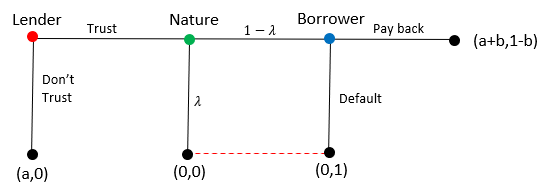
\includegraphics[scale=.4]{figure1.png}
\end{center}

\begin{center}
        \textbf{Table 3: Estimated treatment effects by comparison groups from the Goodman-Bacon decomposition}
        \begin{tabular}{r|ccccccccc}
 & \multicolumn{4}{c}{Post-Nabisco} & & \multicolumn{4}{c}{GM-Quaker} \\ 
 & (1) & (2) & (3) & (4) && (1) & (2) & (3) & (4) \\\hline&&&&&&&&&\\ 
$\E{p}$ & 0.124 & 0.124  & 0.124  & 0.124&& 0.125 & 0.125  & 0.125  & 0.125 \\ 
Med($p$)& 0.122 & 0.122 & 0.122 & 0.122&& 0.123 & 0.123  & 0.123  & 0.123 \\ 
Var($p$)& 0.001 & 0.001 & 0.001 & 0.001&& 0.001 & 0.001  & 0.001  & 0.001 \\
 &&&&&&&&&\\ 
$\E{s}$ & 0.029 & 0.020  & 0.020  & 0.017&& 0.030 & 0.020  & 0.020  & 0.016 \\ 
Med($s$)& 0.013 & 0.011 & 0.011 & 0.009&& 0.016 & 0.011  & 0.011  & 0.009 \\ 
Var($s$)& 0.002 & 0.001 & 0.001 & 0.001&& 0.002 & 0.001  & 0.001  & 0.001 \\
 &&&&&&&&&\\ 
\end{tabular}
\end{center}

\end{document}